%!TEX root = thesis.tex

\chapter{Modelling Spatial Knowledge}
\label{chapter:SpatialKnowledgeChapter}

\section{Introduction}
\label{intro}

How humans gain and store knowledge of their surroundings has been an area of research for several decades now. A significant amount of research has been conducted in trying to understand how way-finding is done using this knowledge. However, how people explore an unfamiliar environment and the interaction between exploration and memory during this process is still an open question. With the increasing number of shopping malls, airports, high rise office buildings and residential towers, there is an increasing likelihood that the occupants of a building may not be regular visitors and as a result will have very little knowledge of the layout. In such a situation, if there is a need to evacuate the building, it is important for planners to know how the occupants would react and find their way to the emergency exits.

Understanding how people navigate and explore unknown spaces is scientifically challenging. One of the primary reasons is that experimentally studying such processes  is difficult and time consuming. Even once an experiment is designed it is always difficult to scale the experiments to many participants and therefore account for various forms of bias due to sampling issues. In recent years serious games (or gamification) have been used in various forms~\cite{npelechano:2008ug, Anonymous:2011ba, Bode06022014} to  provide controlled, yet realistic environments on which to conduct medium to large-scale experiments of human crowd behaviour. We adopt this same methodology in this paper to gain an understanding of how humans with no knowledge of an environment explore. We do this by developing a novel way of identifying the role that memory and {\em non-randomness} plays in human exploration. This method involves experiments where participants play an exploration game, in which they are asked to explore a multi-storey building and complete certain tasks within a certain time limit. All the movement and actions of the players were logged and analyzed for patterns. The main motivations of this analysis were to determine:

\begin{enumerate}
\item Whether memory plays a role in exploration.
\item How memory influences exploration efficiency and an individuals ability to navigate within an environment.
\item If there are common strategies used by humans to explore unknown environments.
\end{enumerate}

The remainder of this paper is organised as follows: Section~\ref{sec:literature_review} provides an overview of our current cunderstanding of how people gain spatial knowledge and do indoor wayfinding. Following this, the game and experiment are described in Section~\ref{sec:experiment_performed_minecraft} and Section~\ref{sec:experiment_details}. Finally, the results are discussed in more detail in Section~\ref{sec:analysis_of_experiment_results}.

\section{Literature Review} % (fold)
\label{sec:literature_review}

Human exploration of indoor environments is a complex process that depends on the perception of the environment, the person's existing knowledge and cultural factors. Before looking at existing models of human exploration it is useful to establish a basic knowledge of how spatial knowledge is stored, used and updated in the human memory. In the context of this paper, it is also useful to understand the methodology used in studying human spatial memory as both an inspiration and validation for the methodology used here.
\subsection{Working Memory} % (fold)
\label{sec:spatial_information_in_human_working_memory}


Since Hebb's seminal work on human memory~\cite{DOH1949}, it's been generally accepted that human memory has a Short Term Memory (STM) component and a Long Term Memory (LTM) component. Baddeley's model of working memory~\cite{BaddeleyHitch74}, which is a three component model consisting of the central executive, a visual spatial sketchpad and a phonological loop is currently one of the most popular models of the working of human memory. Central to this idea is the concept of working memory. Working memory consists of both a visual and a verbal component both of which are limited in capacity.


Linberg and Garling~\cite{lindberg1981acquisition} presented people with tasks to compltete while at the same time performing way finding. Their findings supported the notion that navigation may require effective use of a limited capacity cognitive sub-systems. Several studies~\cite{Garden1992, meilinger2008working} involved experiments examining the way in which way-finding memory was stored. They discovered that when maps were used for learning, only the visuo-spatial component of memory was used. However, in the real world, they found that all the senses were used together and verbal, visuo-spatial, temporal, auditory and even olfactory cues were used by the participants. This suggests that experiments studying way-finding should be as immersive as possible to reflect reality.


Evidence suggests that salient (distinctive) cues are important for place learning. Especially as people grow older and can only perceive and process fewer cues~\cite{Davis01122009} or if the wayfinders are under stress or time pressure~\cite{Ozel:2001tn}.
This is because stress and old age can reduce the working memory capacity. A decreased working memory capacity implies a smaller amount of environmental information is processed and less information is eventually encoded. This in turn implies that only cues that have high perceptual, cognitive or contextual salience are perceived~\cite{Davis01122009}.

\subsection{The building blocks of spatial knowledge} % (fold)
\label{sub:how_people_gain_spatial_information}

There are different scales at which locations are stored in the human mind. This can broadly be divided into 3 levels: Figural Spaces (Object Sized Space), Room Sized Space (Vista Sized Space), Environment Space (Map Sized Space). The approaches used to study these different scales are different~\cite{Sholl:2004vu}. In this research, we only consider Vista and Map sized spaces.


One of the earliest and most influential works on how humans gain and store knowledge of space was Lynch's \emph{The Image of the City}~\cite{lynch_image_1960}. He coined the term \emph{mental map} which refers to a person's perception of the world around him. Perhaps the most important contribution of this paper was the proposal of the fundamental building blocks of a mental map: paths, edges, districts, nodes and landmarks. Paths are routes along which people move, districts are distinct regions, edges define the boundaries between these regions, nodes and landmarks are locations that are points of reference in the mental maps.

How these blocks form a person's image of space was further explored by Siegel and White~\cite{Siegel19759} through their experiments on map learning in children. They proposed a hierarchical model with three distinct parts. They found out that people first gain a knowledge of the \emph{landmarks} in an area, subsequently they learn \emph{routes} connecting these landmarks and finally they gain \emph{survey knowledge}, wherein they have an overall map of the region to the extent that they can determine shortcuts and best routes. They further postulated that adults, despite not having the limitations of a child, mirror a similar process in forming their memory of space.


 Ishikawa and Montello~\cite{Ishikawa200693} emphasized that different people have different abilities and techniques for formation of spatial knowledge. Significantly, they found out that given repeated exposure to the environment, some people were inherently good and other inherently bad at forming and using spatial knowledge.

 Contrary to Siegel and White, they and others~\cite{Moeser01011988} also argue that people's route knowledge and knowledge of space does not improve much after first being formed. More interestingly they found out that certain routes are learned and these routes do not change much, however, inter route connections improve as experience increases.

 In summary, while people do have different techniques of forming and storing spatial knowledge, most studies have confirmed that there is a definite pattern in which it is formed with landmarks and routes playing a key role at the beginning. Furthermore, studies have also shown that this initial knowledge of routes does not change much with time. This indicates that how people first explore an environment probably plays a key role in determining the route they learn and use even in the longer term. Thus motivating the need to understand better the way in which humans explore environments

% subsection the_pioneering_work (end)
\subsection{Indoor Way-finding} % (fold)
\label{sec:indoor_wayfinding}


Kuipers~\cite{Kuipers78} believed that people walk in the general direction of their destination and rarely get lost. However, this is not possible in indoor environments where dead ends are much more common~\cite{HolscherBMS06}. In fact, there are several such differences between indoor and outdoor environments. However, literature on human behavior in internal environments in general, is much more limited. Best~\cite{best1970direction} was the earliest to identify that the number of choice points, i.e. locations where directional changes occurred, was the relevant measure for assessing way finding difficulty, as apposed to to simple metric distances.

Weissman~\cite{Weisman01031981} defined visual access, degree of architectural differentiation, signs and floor plan configurations as the factors that determine way-finding difficulty. \emph{Visual Access} which, in essence, refers to the fact that an environment's external structure gives clues to the internal layout and hence visual access to the outside can decrease way-finding difficulty.

Garling et al.~\cite{garling1983orientation} confirmed the findings about familiarity and visual access. Evans et al.~\cite{evans1980cognitive} discovered that distinct wall colors reduced wall finding complexity. Thorndyke~\cite{Thorndyke1980} found out that experience does improve way-finding but over the period of months rather than hours.

According to~\cite{Gopal1989309}, paths with more choice points, intersections or simply turns are considered more complicated than paths with fewer turns. This is a natural consequence of the fact that there is a higher chance of error. More interestingly, they state that paths with more turns are perceived to be longer as well.

Holscher et al.~\cite{HolscherBMS06} explored the various strategies that people use in exploring multi-storey buildings. The first strategy shown by Kuipers et al.~\cite{Kuipers01012003} stresses on the primacy of a set of central paths or a \emph{route skeleton} in way finding. People explore along this central route skeleton. Another strategy referred to as the \emph{horizontal position strategy} was rarely used by people and was generally not very efficient. Here people try to get to the correct horizontal location first. Following this they try to find the way to the correct floor. The reduced efficiency of this strategy was a natural consequence of the fact that the experiments in the paper were conducted in a building where each floor was different from the next. The last strategy which was used by more experienced participants and was also proved to be the most efficient is what was called the \emph{floor first strategy}. As the name suggests, this strategy involved the person trying to get to the required floor first and then exploring horizontally to find the goal.

O'Neill~\cite{O'Neill1992319} studied the accuracy of simulated environments in studying way-finding behavior. Their approach was to examine behavior in a simulated environment and compare it to results from actual experiments. Their findings showed that human behavior in simulated environments reasonably mimicked real life. Montello et al.~\cite{Montello:2004uj} had a much more comprehensive analysis of the effect of different sources: maps, virtual environments and real world experience. In general, the more immersive the environment the less difference there is from real life. % Can't find MJ ROsama paper

% section literature_review (end)

\section{Experiment Performed} % (fold)
\label{sec:experiment_performed_minecraft}

In order to understand more about how humans explore environments and store spatial knowledge, we created a game that requires  exploration and way-finding and analysed how the game was played. The environment must have some degree of complexity or diversity to be engaging and invite exploration~\cite{kaplan1983cognition}. To reduce development effort and to allow for flexibility in environment creation, we built the experiment inside the popular game Minecraft.

\subsection{The minecraft gaming environment}
\label{sec:the_minecraft_gaming_environment}

Minecraft~\cite{Minecraft} is a java based multi-platform sandbox construction game. The game involves players creating and destroying various types of blocks in a three-dimensional environment. In the original game, the player takes on an avatar that can destroy or create blocks, forming buildings, structures, artwork and even entire cities on multi-player servers or single player worlds across multiple game modes.



In the original game players can break any block and build any block provided, he/she has the resources. In the work for this paper, we used an existing plugin~\cite{BukkitPermissions} that constrained players so that they could only move around in the environment and interact with doors and switches i.e. elements that were essential for the experiment. A second modification was created~\cite{MyStatisticsPlugin} to keep a log of the movements and actions of the players and store them in a MySql server for analysis. The following sections describe the game, the methodology used for analysis and some of conclusions from the experiments.



\subsection{The game}
\label{sec:the_game}

The literature review covered some different ways in which simulated environments have been used for studying human spatial knowledge. These simulated environments ranged from VR environments to very simple games of finding a way through a maze. Most experiments tried to constrain the first part of knowledge acquisition. A typical example is Melinger Knauff and Bulthoff~\cite{meilinger2008working} who ensured that all particiapnts got indentical stimuli in order to be able to fairly compare secondary task comparison. So participants watched a video rather than actively navigating through the environment. This has resulted in there being very little existing literature on how people actually explore environments; also, we believe that the paths taken during exploration could also reveal interesting aspects of human exploration.


The premise of the game is that player has been teleported into an old abandoned palace where eleven people have been imprisoned in different locations spread over the three storey environment. The objective of the game is for the player to free the eleven prisoners and subsequently follow instructions to open the main gate to the palace and escape. The palace is a three storey building with 44 rooms modified from an existing Minecraft map~\cite{RoyalPalaceMap}. The layout of each floor of the palace is shown in Figure~\ref{fig:FloorPlans}. A player joining the server is spawned at the location indicated on the map with an X. During the first few minutes the player is presented with the story line and interactively told how to use the controls and play the game and free the first prisoner. Subsequently, the player is tasked to find and free the other prisoners. The locations of the prisons, as shown by the shaded areas in the map, are spread all over the building. This is the first phase of the game and we call this the \emph{exploration phase}. This phase requires the player to move around and explore the building. This phase can be reasonably equated to what a new visitor to a building (e.g., shopping mall) experiences.



\begin{figure}[!tb]
  \centering
   % \subfloat[Ground Floor]{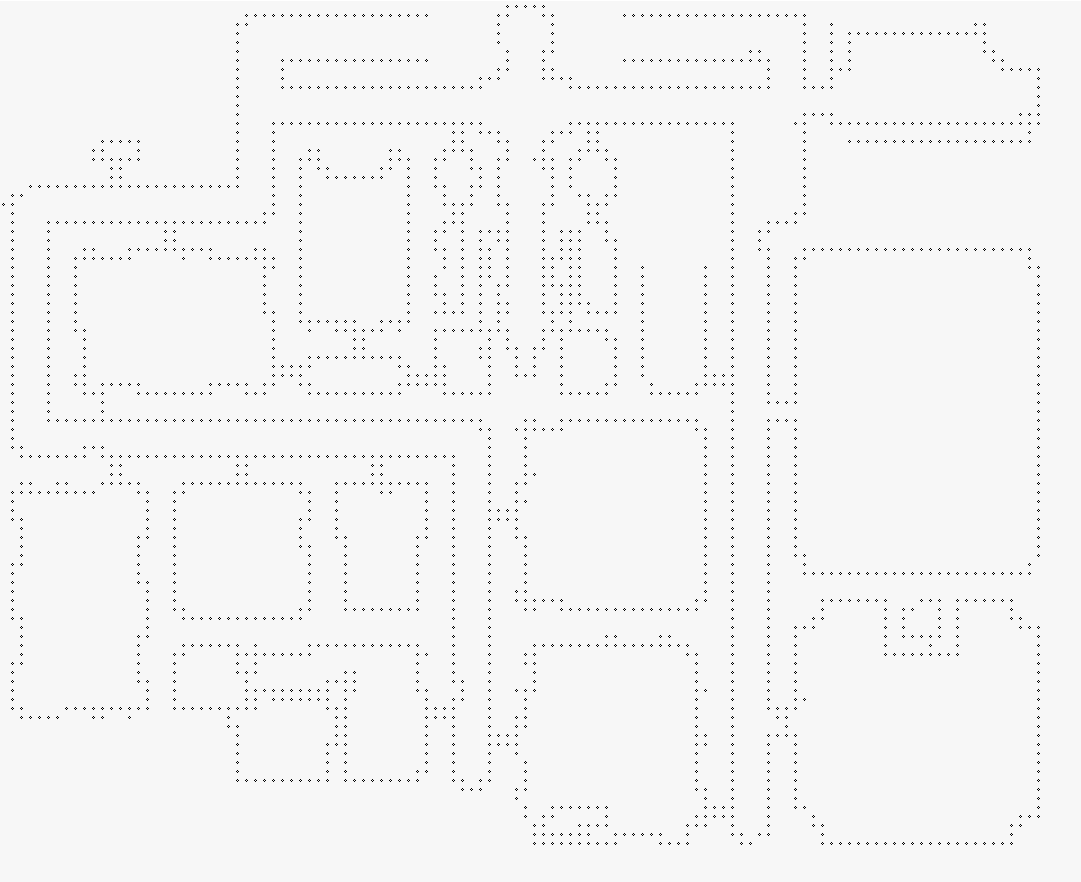
\includegraphics[width=6cm, height=3cm]{floor0}}
   %  \hspace{1pt}
    \subfloat[Ground Floor]{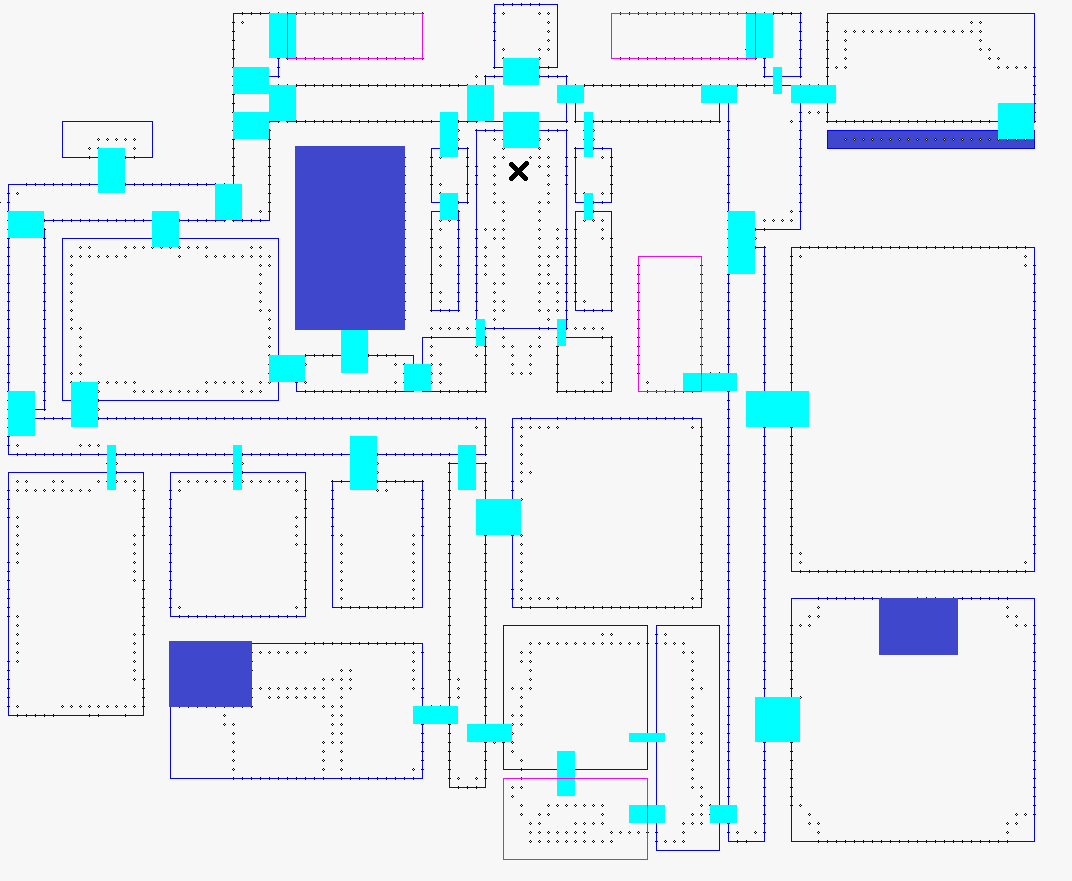
\includegraphics[width=6cm, height=3cm]{floor0WithRooms}}
   \\
  %  \subfloat[First Floor]{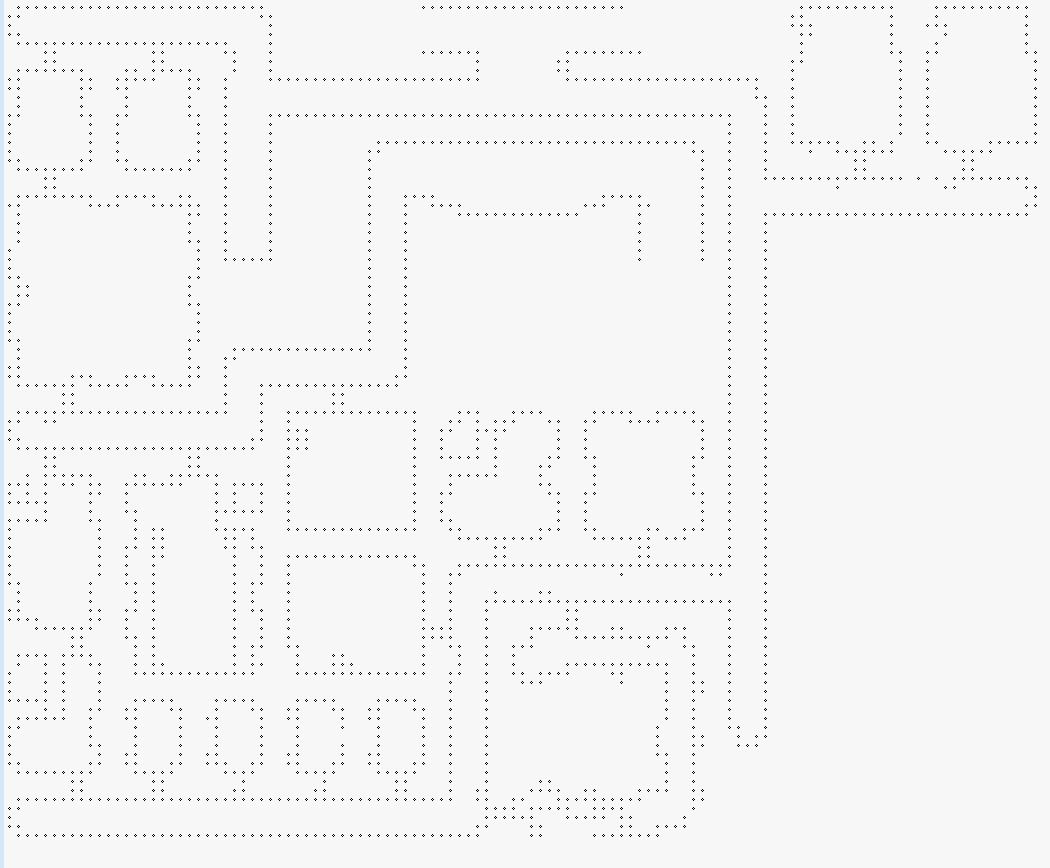
\includegraphics[width=6cm, height=3cm]{floor1}}
  % \hspace{1pt}
    \subfloat[First Floor]{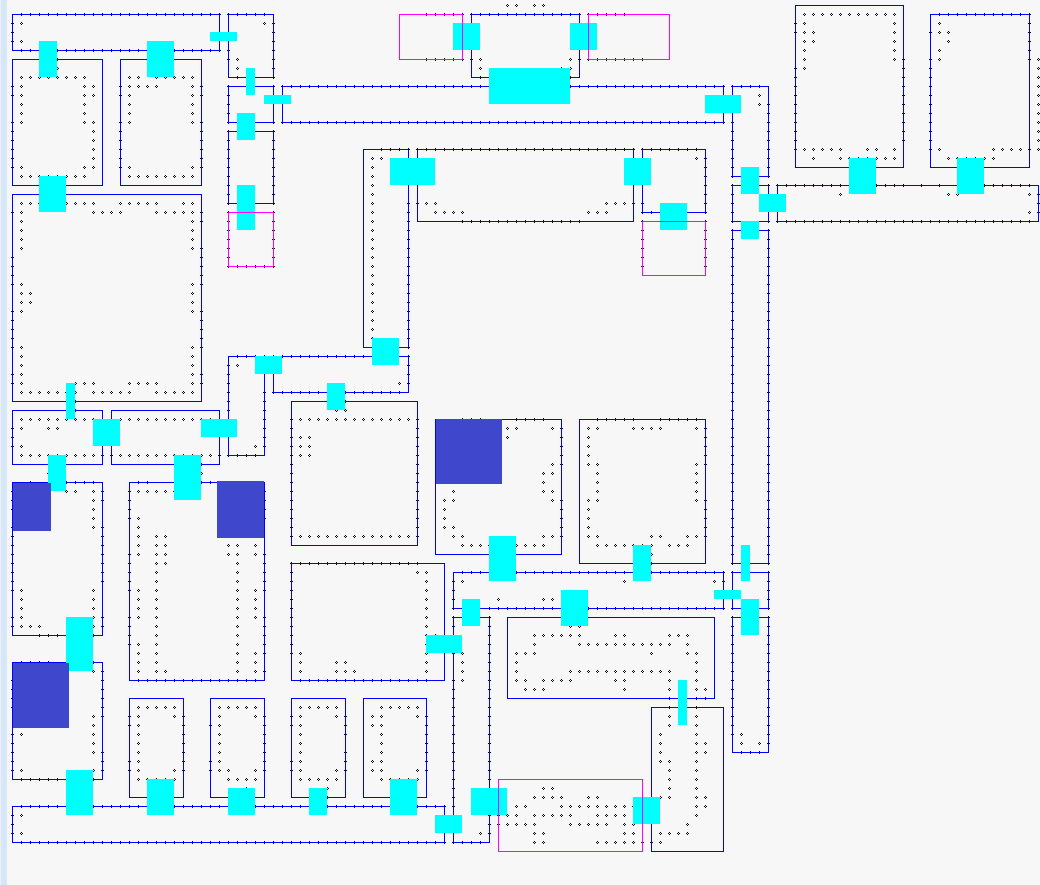
\includegraphics[width=6cm, height=3cm]{floor1WithRooms}}
  \\
  % \subfloat[Second Floor]{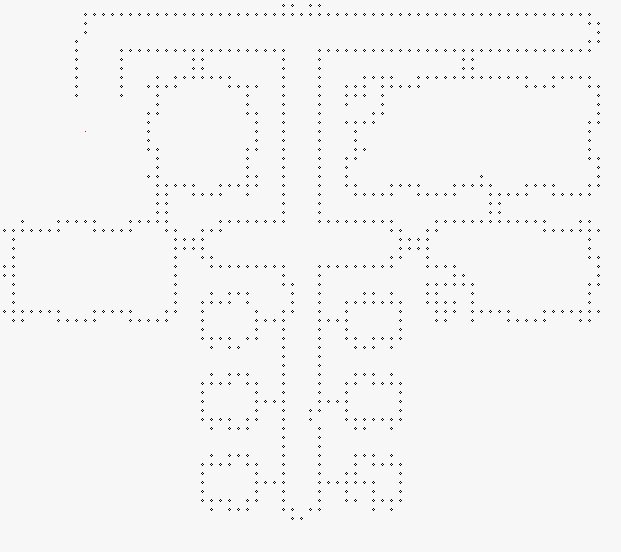
\includegraphics[width=6cm, height=3cm]{floor2}}
  % \hspace{1pt}
  \subfloat[Second Floor]{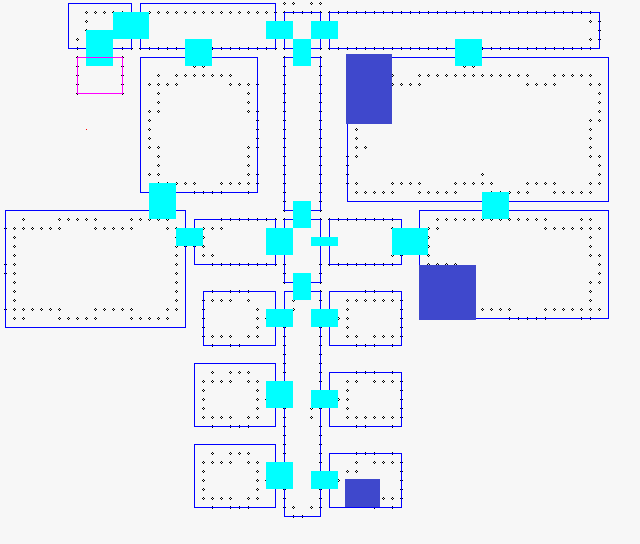
\includegraphics[width=6cm, height=3cm]{floor2WithRooms}}
  \caption{Floor Plans of the three floors. The X indicates the starting point. The blue color indicates the prisoner locations.}
  \label{fig:FloorPlans}
\end{figure}



The next phase, which we call \emph{knowledge testing phase}, starts when the eleventh prisoner has been freed. During the phase, the cognitive map formed by the player is tested through a series of three tasks. By not revealing the nature of the second phase to the player at the beginning of the game and also by hiding the location of the knowledge testing tasks, we ensure that the player does not make a special effort in remembering locations which could artificially alter the cognitive map formed.

When the eleventh prisoner is freed and the exploration phase ends, the player is given instructions to proceed to the gallery room in the building. This room would have been examined by the player during exploration. It is the only room in the palace whose walls are covered with paintings and this makes it reasonably likely that the player will remember this location because of its \emph{perceptual salience}~\cite{Davis01122009}.
% Majority of the players remembering this location indicates that perceptua is indeed a key factor in remembering locations.

Once the player locates and presses the switch that is revealed in this room, the player is given instructions to the second floor library. There are two important factors for having this particular location. Firstly, the library has four entrances and is very likely that the player would have entered this room multiple times during the exploration phase. Secondly, being on the second floor, there are multiple paths to this location from the gallery as can be seen in figure~\ref{fig:UnscaledMap}. Preference for a particular route among players would help understand more about his/ her cognitive map.

Once the player finds this location he is given the final instruction to proceed to his starting location to find the final switch that will open the main gate to the palace. Again, there are multiple routes to this location some of which are significantly shorter than others. Also, being a starting location and in a somewhat central location the location will likely have been frequently visited and will have some \emph{cognitive salience}~\cite{Davis01122009}.

The player locations at different times and the time at which each prison was opened and the time taken to complete each task in the testing phase were all recorded. The next section outlines the details of the experiment itself.


\section{Experiment details} % (fold)
\label{sec:experiment_details}

There were 50 participants in all. Each participant was given five minutes to get used to the controls of the first person game which involved using both the mouse and the keyboard: W, A, S and D keys for movement and the mouse for looking around. A single click on the mouse would allow the player to interact with the environment by either opening doors or prisons. The players were given 45 minutes to complete the game. Of the 50 participants, the data from only 44 participants were used, the remaining six experienced motion sickness from the movement in the first person gaming environment and had to quit playing before the game could be completed.

% section experiment_details (end)


\section{Analysis of Experiment Results} % (fold)
\label{sec:analysis_of_experiment_results}

In this section we introduce some of the metrics that were used for analyzing movement in order to understand the role that memory plays in exploration.

\subsection{Calculation of random walks}

\begin{figure*}[!htb]
\centering
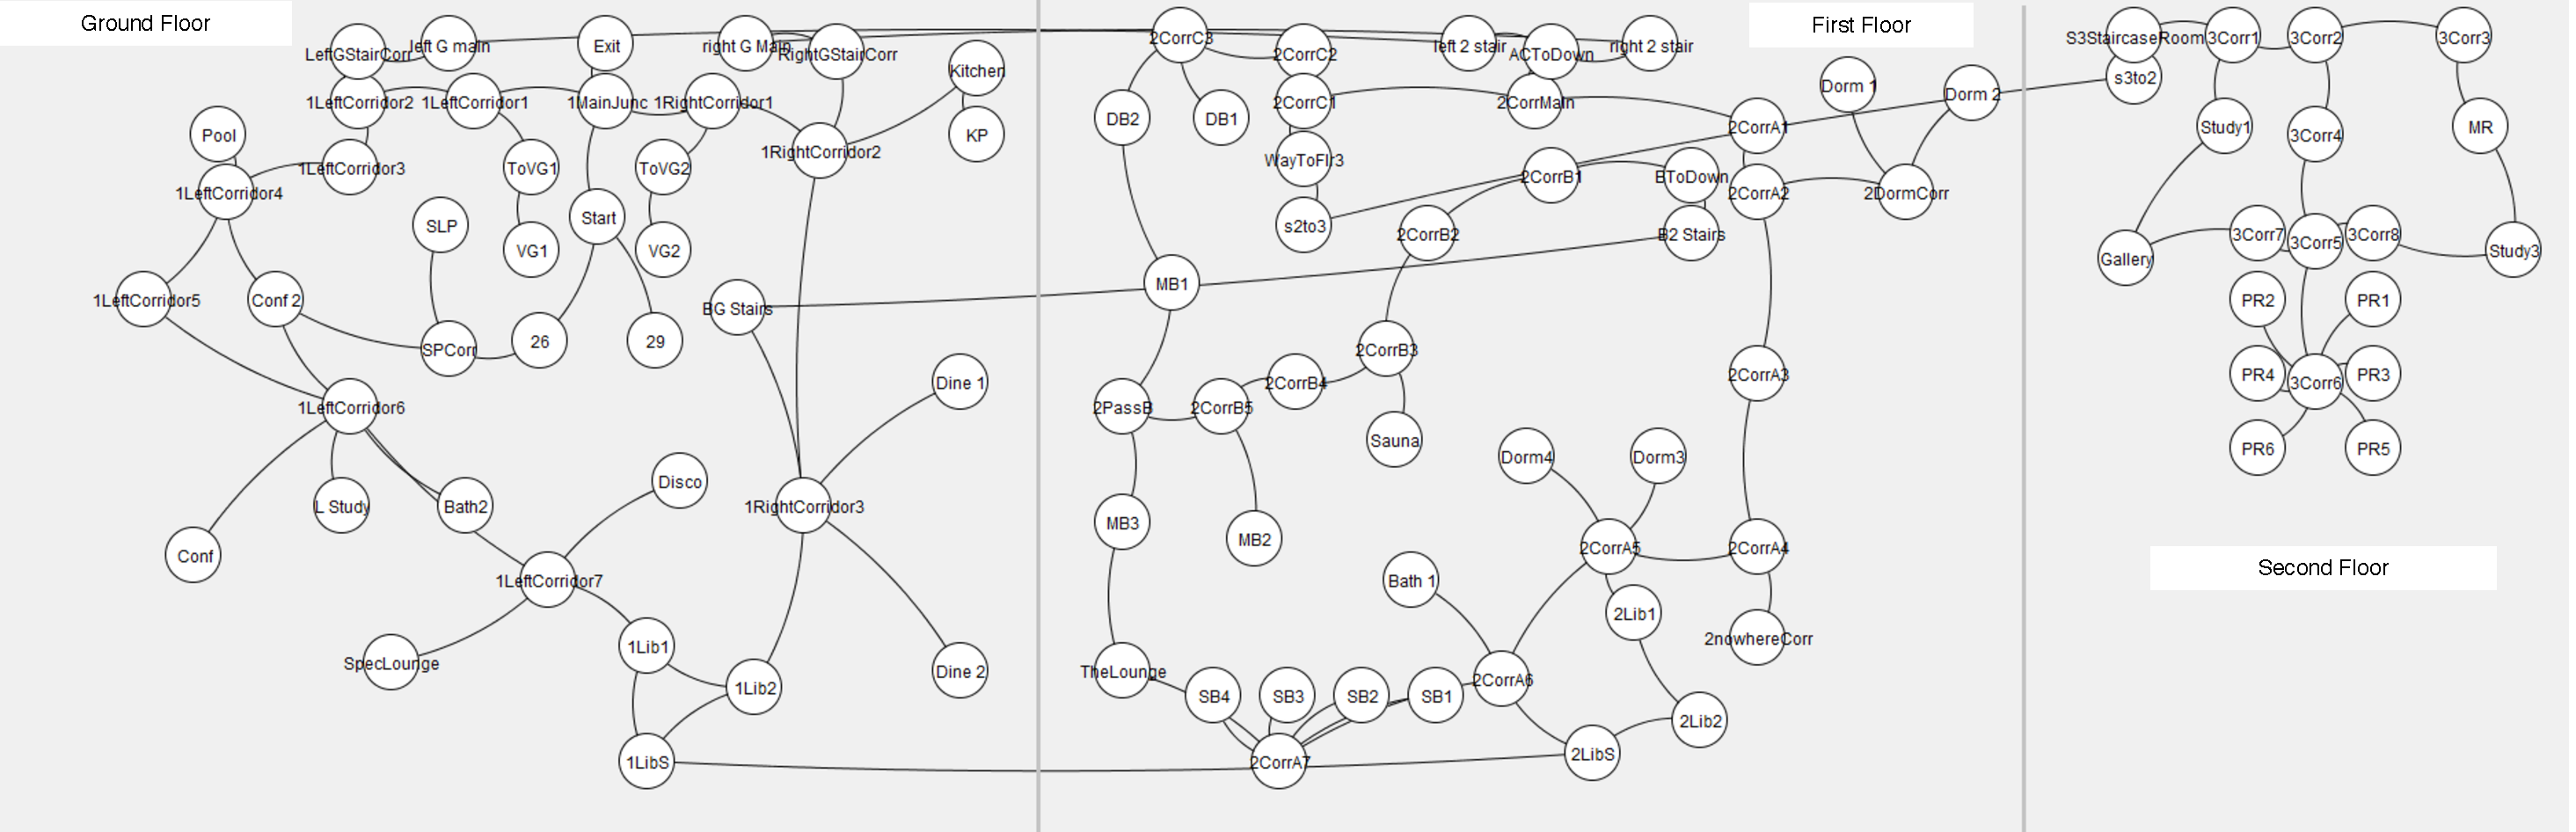
\includegraphics[width=\textwidth]{unscaledRoomLayout.pdf}
\caption{Room Layout Graph}
\label{fig:UnscaledMap}
\end{figure*}

A random walk is used as a benchmark for comparison. This random walk is done on the undirected graph shown in Figure~\ref{fig:UnscaledMap} which is a graphical illustration of the aggregated floor plans from Figure~\ref{fig:FloorPlans}. Each iteration of the random walk is performed until the walker covers 100 percent of the environment. A collection of random walks is obtained until the variance in the radius of gyration of generated graphs stabilizes.


\subsection{Room visit frequencies}


We first calculated the frequency of visits for each room per player and compared this against the random walker. This is a simple test to determine if the players have a pattern or strategy in their exploration.

\subsubsection{Calculation}


For any room $r$, let $f_p(r)$ be the number of times a player visited $r$ and let $f_{rw}(r)$ be the number of times a random walker visited the same room. Then the normalized number of visits by a player to the room can be obtained as:

\begin{equation}
y(r) = \frac{\alpha_p(r)}{\alpha_{rw}(r)}
\end{equation}

Where
\begin{equation}
\alpha_x(r) = \frac{f_x(r)}{\sum_{a \in R} f_x(a)}
\end{equation}

Figure~\ref{fig:scaledMap} shows the value of $y(r)$ each room  as a scaled version of Figure~\ref{fig:UnscaledMap}. Red color indicates a $y$ value of greater than $1.05$ and the green color indicates a value of less than $0.95$. The diameter of each node in this graph is scaled to $y_r \times (unscaled\ diameter)$.



This implies that, a white color indicates that the normalized number of visits is the same in both random walk and in the data. A value greater than 1 indicates that players visited the more than the random walker and smaller value indicates the opposite. It is hard to discern any pattern in this data other than that the amount of time spent on the third floor is higher than the number of visits on the second floor which is more than the number of visits on the first floor.


\begin{figure*}[!htb]
\centering
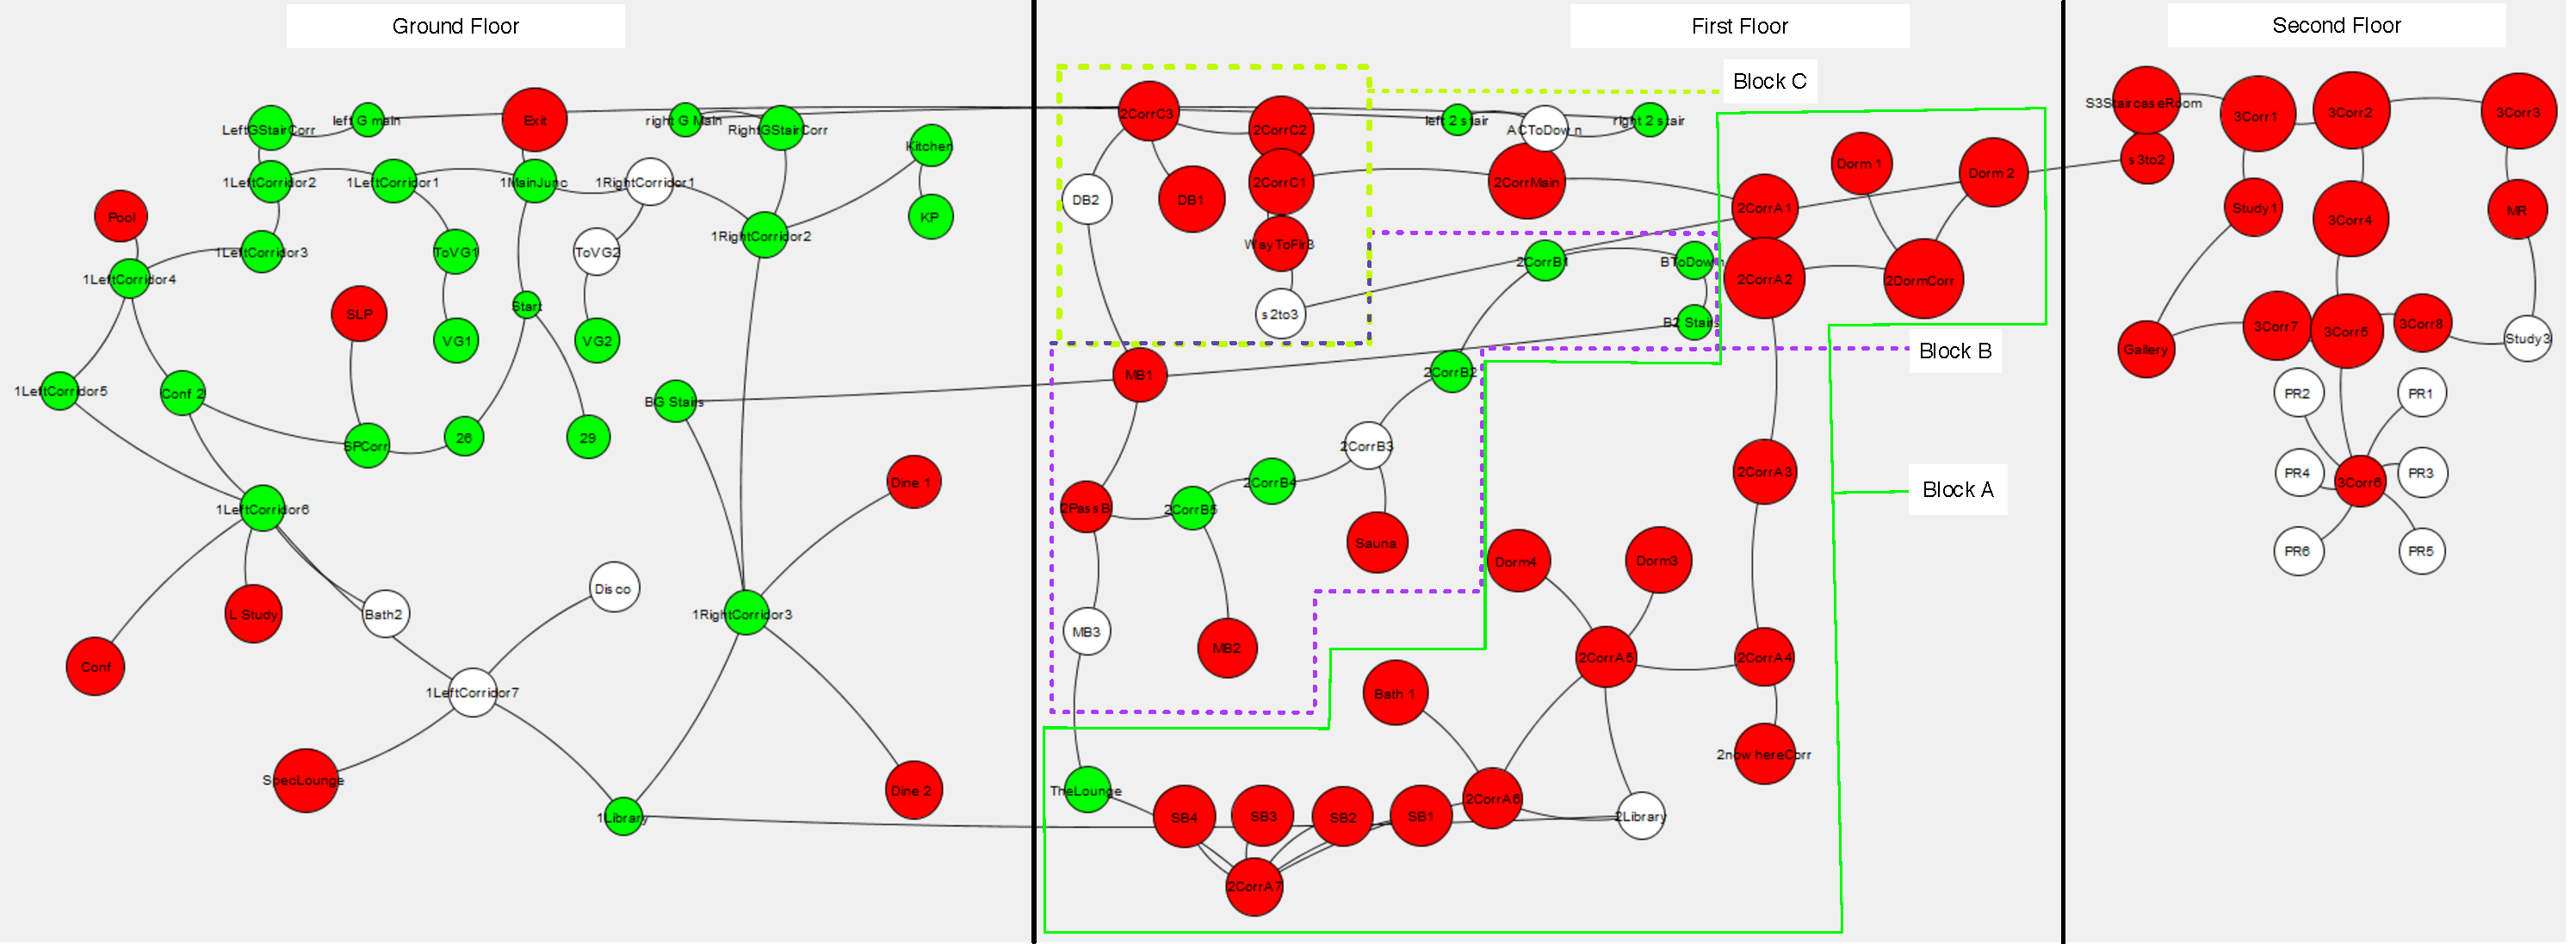
\includegraphics[width=\textwidth]{scaledGraph.pdf}
\caption{Map scaled by normalized number of visits}
\label{fig:scaledMap}
\end{figure*}

As it can be clearly seen that players seem to have a lot more visits on the third floor, we decided to normalize to number of visits on the floor rather than the total number of visits. On doing this, if the graph turned out to be different, it would seem that unlike a random walker, a player differentiates between a simple link between rooms or corridors and a staircase which is a link between floors. Figure~\ref{fig:scaledGraphByFloor} is the floor normalized version of Figure~\ref{fig:scaledMap}.


\begin{figure*}[!htb]
\centering
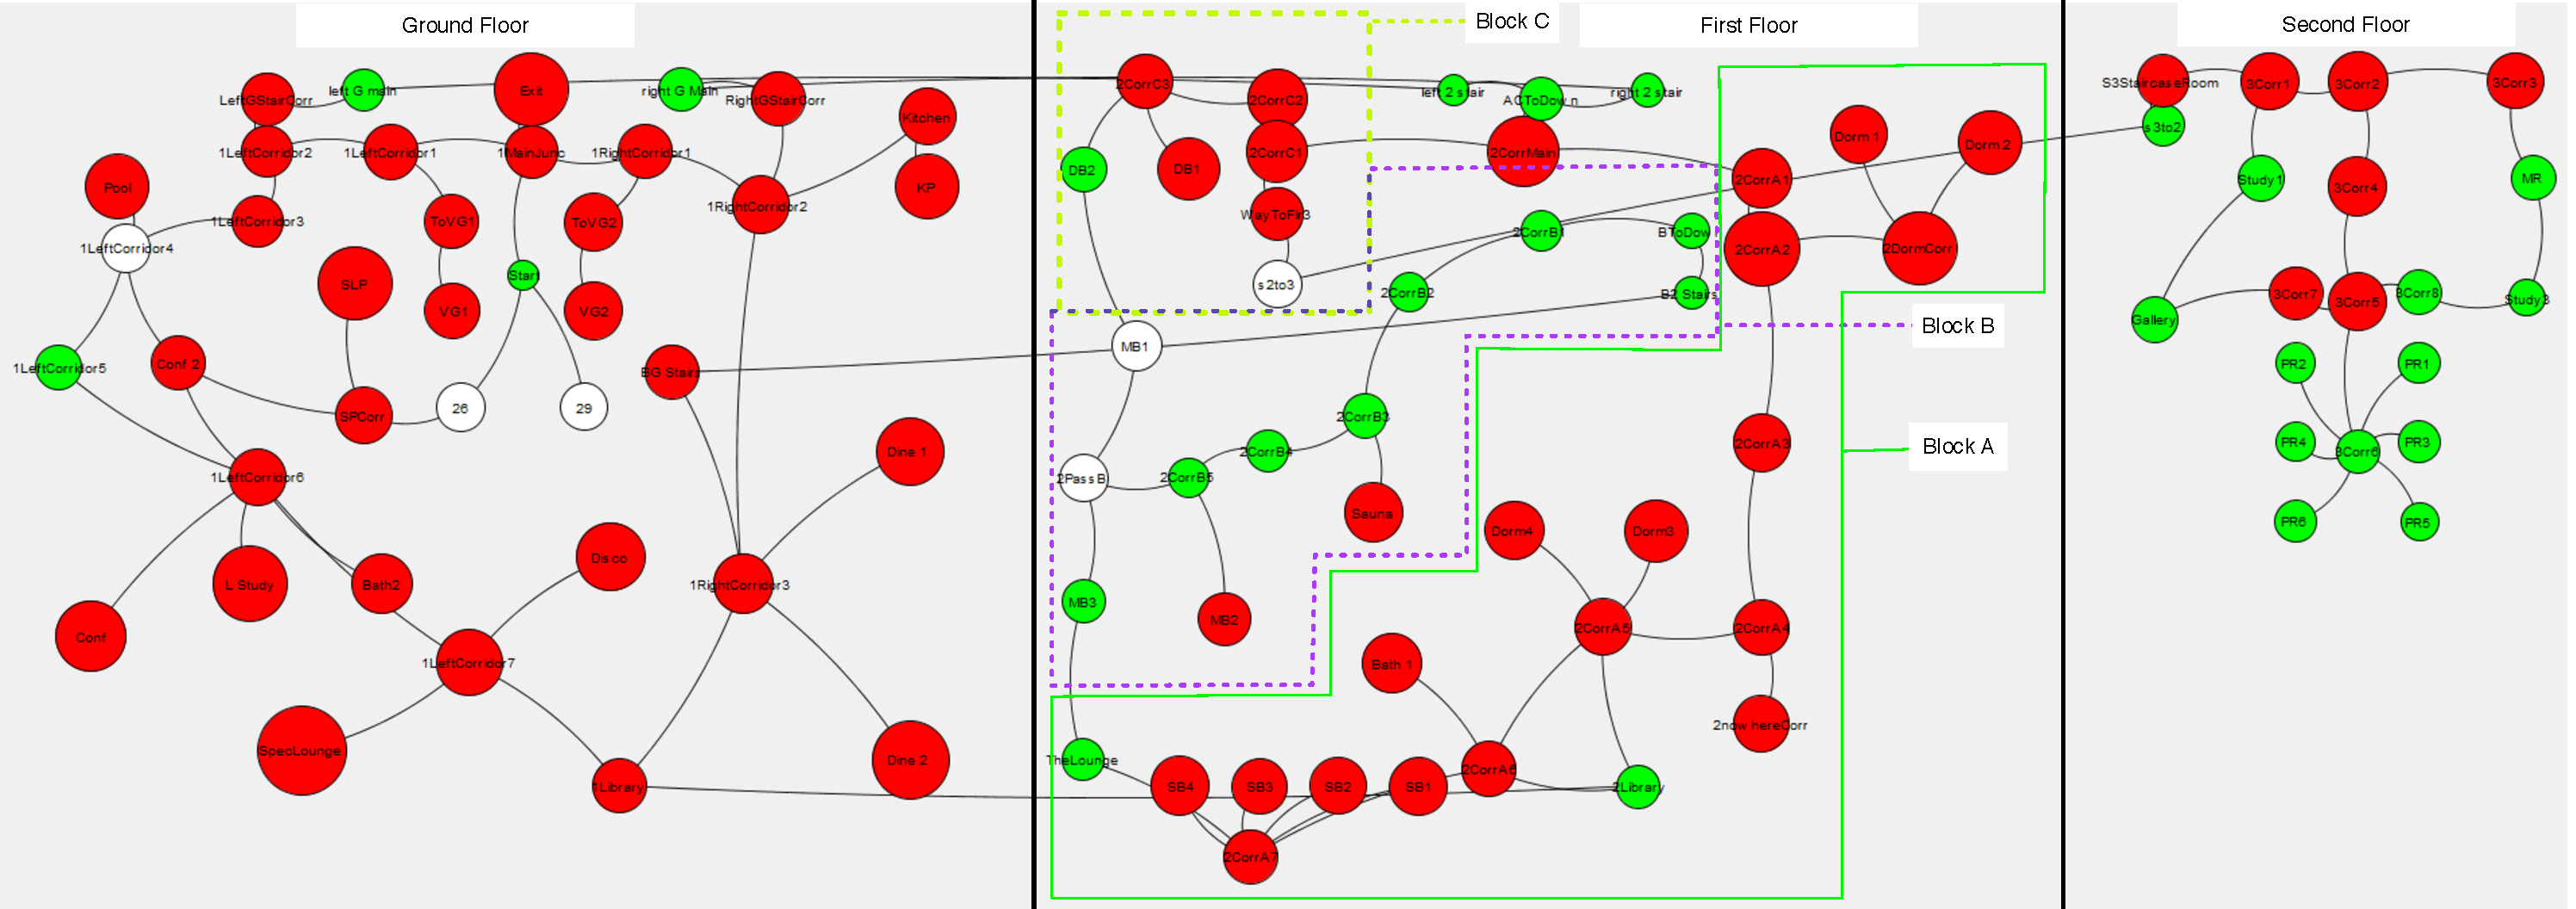
\includegraphics[width=\textwidth]{scaledGraphPerFloor.pdf}
\caption{Map scaled by floor normalized number of visits}
\label{fig:scaledGraphByFloor}
\end{figure*}




\subsubsection{Discussion}

The figures in this section provides a possible validation of a variation of the floor first strategy~\cite{HolscherBMS06} used for exploration. The strategy in the original paper was for way-finding, but here it seems to be being used for exploration. The players seem to consider each floor as a separate entity and are generally reluctant to take the staircase. This is also because the process of separating each floor helps in bringing some organization and structure to the confusing room layout and the process of exploration (i.e., completely explore one level before the next).

The existence of this floor first strategy is further demonstrated by the low visit frequencies to Block B on the second floor. Block B on the second floor is accessible in three possible ways, through a staircase in the first floor and through rooms DB2 and The Lounge in Block A and C respectively. This means that Block B is not accessible via direct corridor from the same floor like Block A and C. The only obvious way is by going down a floor.



\subsection{Markov data analysis}
\label{sec:Markov_data_analysis}


In this section we conduct an analysis of the recorded player data in comparison to biased and unbiased random walkers. The purpose is to investigate the role that memory plays in the exploration of the environment. First we conduct a Markovian analysis of the player data collected to understand the role of memory in the efficiency of the exploration process.

We take an $m^{th}$ order Markov model to represent an $m$-step memory of the explorer, where steps constitute room visits. One way to speculate on the size of the memory used by a human during exploration is to predict a path of length $n$ from some Markov data of order $m < n$.

In an $m^{th}$ order Markov model, the basic idea is the action at any point of time depends only on the previous $m$ actions. By assuming that the process of exploration is an $m^{th}$ order Markov process, we are hypothesizing that the next room that is visited by a player is only dependent on the previous $m$ steps. This is different from a simple random walker that tries to avoid the previous $m$ rooms. Since the next step is dependent on the actions of players who have visited that same subsequence of $m$ rooms, the Markov model theoretically encapsulates other factors like layout, visibility, etc. The methodology of doing this Markovian analysis is explained in more detail in Section~\ref{sec:calculation_of_markov_data}.

We then try to understand if an $m^{th}$ order Markov model is sufficient for describing exploration efficiency. We do this by measuring the exploration performance in terms of minimum hops needed and maximum coverage obtained for different values of $m$ and  comparing this with the exploration of a random walker and an agent-based model that uses a simple memory rule for exploration. Interestingly we find significant performance improvements when we reach $m$ of 6 to 8.

\begin{table*}[!tb]
\caption{Summary of symbols and their meaning}
\begin{tabular}{p{1.5in}p{5in}}
\tabularnewline
\hline\hline %inserts double horizontal lines
Symbol & Meaning \\
\hline
$Pr (A|B)$ & Probability of occurrence of event A given event B \\
$X_n$ & Random variable indicating the location in the $n^{th}$ step \\
$p^{(n)}_{ij}$ & Probability of going from state $i$ to state $j$ in $n$ steps \\
$R$ & Set of all rooms \\
$r$ & A particular room \\
$N_r$ & Set of neighbours of room $r$ \\
$P^{(n,D)}$ & Set of all paths of length $n$ in dataset $D$\\
$Q^{(n)}$ & Random variable representing a path of length $n$\\
$q^{(n)}$ & A particular path of length $n$\\
$\phi(a,S)$ & The frequency of element $a$ in set $S$\\
$x^{(q)}_{i}$ & $i^{th}$ location in a particular path $q$\\

\hline
\end{tabular}
\label{tab:Symbol_Table}
\end{table*}


\subsubsection{Calculation of markov data} % (fold)
\label{sec:calculation_of_markov_data}


This section explains how the aforementioned Markov calculations are done. These calculations are performed on the data that was derived from the experiments in Minecraft. This data is stored in the form of a directed graph with each node corresponding to a room and a directed edge indicating the movement of the player from one node to the next. Each edge also stores the time of traversal.


The $n^{th}$ order Markov probability of visiting a room $b$ from a room $a$ is defined as the probability that the $n^{th}$ room after visiting room $a$ is room $b$. Mathematically, it can be stated as:

\begin{equation}
    p^{n}_{ab} = Pr(X_{n}=b|X_{0}=a)
\end{equation}

It is assumed that it is a time homogeneous process, i.e.,

\begin{equation}
    p^{n}_{ab} = Pr(X_{k+n}=b|X_{k}=a) \ where\  k \geq 0
\end{equation}



We can calculate the $n^{th}$ order Markov data of a particular dataset using the following :
\begin{enumerate}
    \item For each path of length $n$, the number of times that path is observed in dataset $D$. This can be directly counted from the dataset. From this, equation~\ref{eq:HeatMapEquation} can be used to derive $p^{n}_{ab}$:

    \begin{equation}
        p^{n}_{ab} = \frac{\left\vert{P^{(n,D)}_{ab}}\right\vert}{\sum\limits_{x\in R}\left\vert{P^{(n,D)}_{ax}}\right\vert}
        \label{eq:HeatMapEquation}
    \end{equation}

    \item For each path of length $n$, the likelihood that a particular path is the result of $n$ steps being taken.
    % Each row corresponds to a particular path of length $n$. To avoid unnecessary wastage of memory, paths and destinations that are not taken and thus have 0 probability are not stored in the table.
    From the frequency data, it is possible to generate the likelihoods using the following calculation:
    \begin{equation}
        Pr(Q^{(n)}=q^{(n)}) = \frac{\phi(q^{(n)},P^{(n,D)})}{\left\vert{P^{(n,D)}}\right\vert}
        \label{eq:TableEquation}
    \end{equation}


    \item We finally calculate the the probability of any destination given a particular path of length $n$. Mathematically, this gives $Pr(X_{n+1}=r|q^{(n)}) \forall r \in R$.

\end{enumerate}


Given the probability of any destination, given a particular path of length $n$, it is possible to predict the $(m+1)^{th}$ step given the previous $m$ steps i.e. the $1^{st}$ to $m^{th}$ step. Following this, the $(m+2)^{th}$ step can be predicted by doing the same calculation using the previous $m$ steps from $2$ to $m+1$. Thus any path of length $n$ can be extrapolated from an $m^{th}$ order data.



\subsubsection{Types Of Exploring agents}
\label{sec:types_of_data}

To evaluate the role of memory in exploration by comparing the exploration performance of the following:
\begin{itemize}
    \item \emph{Actual Players}: This is the average over the actual paths taken by all the players.

    \item \emph{Markov Agents}: These agents explore the environment using the calculations explained in Section~\ref{sec:calculation_of_markov_data}. As explained there, the action of an $m^{th}$ order markov agent at a particular point in the path is a function of the actions of the actual players who had taken the same $m$ steps. The calculations are performed for m from 1 to 13. We present further analysis on the validity of this calculation in the appendix.

    \item \emph{Unbiased Random Walker}:  The next move is chosen by this agent is chosen randomly with equal probability.

    \item \emph{Agent with $m$-step Memory}: In this, the agent is assumed to have a $m$-step memory. It moves exactly like the random walker except that it avoids moving back to any of the $m$ rooms it visited previously. If there is no unvisited room, the agent checks it's $m$-step memory for an unvisited junction. If such a junction exists, it goes back to that point and continues exploring. If such a junction does not exist, then the agent choses a location at random with equal probability.

\end{itemize}

% section types_of_data (end)

\subsubsection{Expected Coverage Given Number Of Hops} % (fold)
\label{sec:calculation_4_expected_coverage_given_number_of_hops}

The average coverage after a given number of hops gives an estimate of the efficiency and effectiveness of exploration. Figure~\ref{fig:coverage} shows the coverage of the four agents explained in Section~\ref{sec:types_of_data} after 300 hops.


\begin{figure*}[tb]
    \begin{center}
        \includegraphics[width=\columnwidth]{coverage-300.PNG}
    \end{center}
    \caption{Coverage for 300 hops}
    \label{fig:coverage}
\end{figure*}


The figure seems to indicate that even a second order Markov agent i.e. one whose next position is only dependent on it's current and previous position performs much better than an unbiased random walker. It also seems to indicate that after 300 hops the performance of the actual players are much better than both the Markov agent and an agent with simple $m$-step memory. This is not surprising since, it is likely that when nearing 300 hops, the long term memory of the player also has a major influence. As mentioned in section~\ref{sec:literature_review}, in the slightly longer term, the walker would probably have formed a route or some sort of survey knowledge and this will include the structure of the building, routes and short cuts and, in general, more structure to the mental map. The fact that the Markov agent performs worse than the agent with memory regardless of the value of $m$ agrees somewhat with this conclusion. However, this could also because the Markov agent has the same errors as the collective human memory - whereas the m-step agent has perfect memory.


% section calculation_4_coverage_given_number_of_hops (end)

\subsubsection{Expected Hops Given Coverage} % (fold)
\label{sec:calculation_5_expected_hops_given_coverage}

We also calculate the minimum number of hops required to obtain a given coverage. It gives a more granular measure than coverage for a given number of hops. The average final coverage for a player after the exploration phase of the game is  $89 \pm 1$ as shown in Figure~\ref{fig:coverage}. We first calculated the minimum number of hops required by the different agents to obtain this coverage (Figure~\ref{fig:hops_for_88_coverage}). This graph shows the number of hops required by different types of agents for getting this coverage. This graph shows the same pattern as discussed in Section~\ref{sec:calculation_4_expected_coverage_given_number_of_hops}.

It is interesting to see how the graph is for $50\%$ coverage. By this point it is unlikely that long term memory will have much of an effect. Figure~\ref{fig:hops_for_50_coverage} shows the results of this calculation. The magnitude of the difference between hops required in for $50\%$ and $88\%$ shows a non linear increase indicating that exploration becomes progressively more difficult. The figure also shows that agents with a simple memory of 5 or more steps seem to perform at the same level or better than humans. It is also interesting to note that the performance Markov agents however, still perform worse than agents with a simple $m$-step memory probably because of the imperfect nature of the short term human memory on which it is based. The gap in performance between the markov agent and the actual player is quite narrow at $m = 7$ to $9$. This indicates that the room visited at any point can be reasonably predicted from the previous 6-8 rooms during this early phase of exploration. However, the fact that the gap exists indicates that this is probably not sufficient to reproduce human exploration.

\begin{figure}[tb]
    \centering
    \subfloat[Hops for 88\% coverage.]{\includegraphics[width=\columnwidth]{hops-88.PNG} \label{fig:hops_for_88_coverage}}
   \\
   \subfloat[Hops for 50\% coverage]{\includegraphics[width=\columnwidth]{hops-50.PNG}\label{fig:hops_for_50_coverage}}

    \caption{Minimum hops required for obtaining given coverage}
\end{figure}

% section significance_of_hops_and_coverage_calculation (end)




\subsection{Empirical Analysis} % (fold)
\label{sec:empiricalanalysis}

We performed a empirical and qualitative analysis of the actions of the players at different locations. This analysis revealed the existence of definite decision points, patterns in exploration and the importance of cues in recognition and memory.



\subsubsection{Existence of decision points} % (fold)
\label{sec:definite_decision_points}

Figure~\ref{fig:simpleCorridorBehavior} illustrates the decisions of people at different types of rooms and corridors, where it is possible for them to make a decision. At certain locations, such as corridors that have no rooms on the side (i.e. they are simply connections between two areas), staircases and simple corners, the only decision that a player can make is whether to move forward or turn back. Turning back would require a conscious decision by the player. A pure random walker would generally have an equal chance of going back or forward. As clearly shown in figure~\ref{fig:simpleCorridorBehavior}, the data reveals that players generally avoid such decisions.

What is more interesting is the behavior of people at rooms which have just two doors. The data seems to reveal that if the opposite door is clearly visible from one door, then the room is used by the player almost exactly like a corridor, though there is a slightly higher chance of turning back. However, if the opposite door is not visible, then there is a roughly 50-50 chance of the person taking that other door or going back.

\begin{figure}[tb]
    \begin{center}
        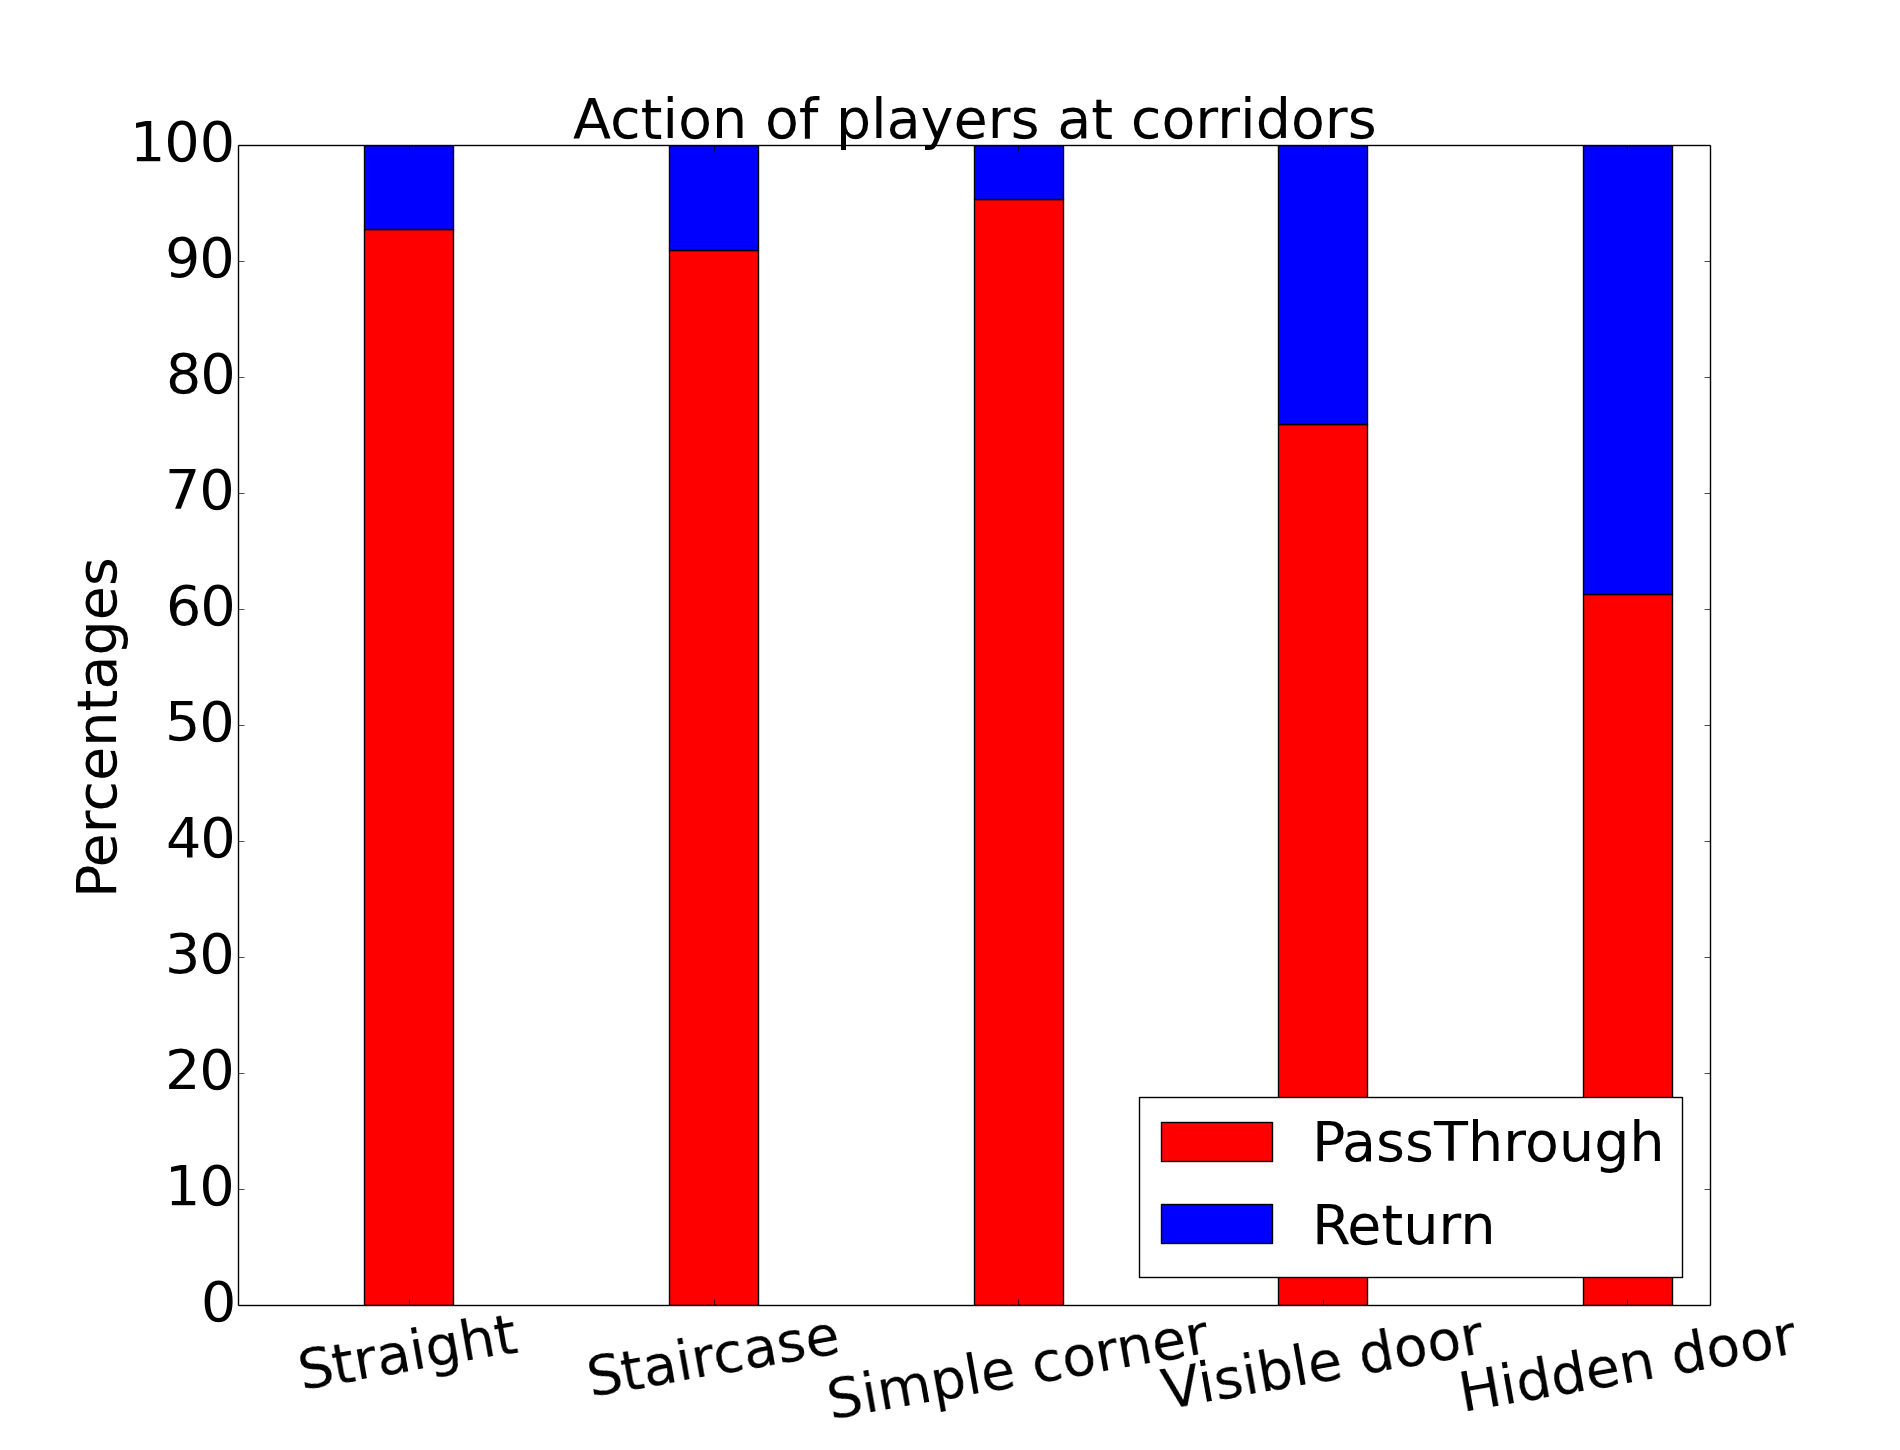
\includegraphics[width=\columnwidth]{simpleCorridorBehavior.png}
    \end{center}
    \caption{Behavior at simple corridors. There are definite decision points during exploration}
    \label{fig:simpleCorridorBehavior}
\end{figure}
% section definite_decision_points (end)

\subsubsection{Location recognition and memory} % (fold)
\label{sec:on_memory_and_exploration}

\begin{figure}[tb]
    \begin{center}
        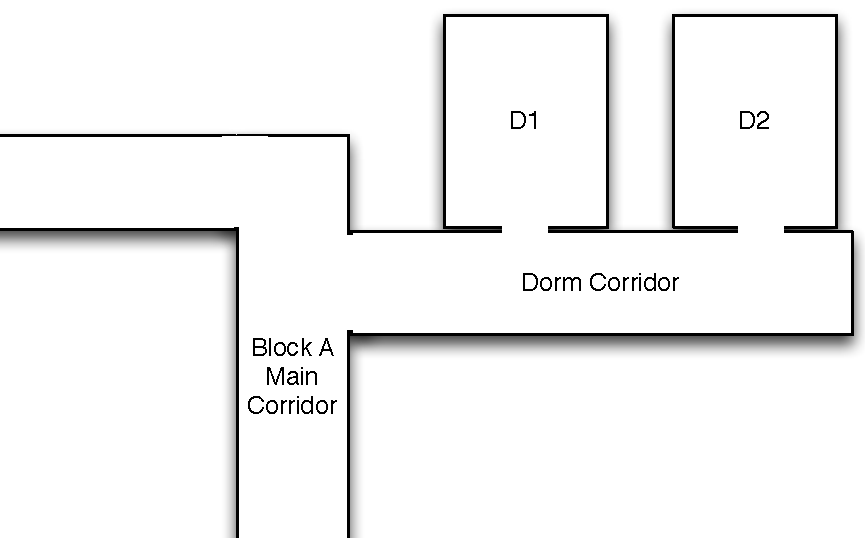
\includegraphics[height=2in]{dormCorrLayout.pdf}
    \end{center}
    \caption{Layout of the relevant corridor}
    \label{fig:dormCorrLayout}
\end{figure}

In the game environment, there exists a corridor that seems to reveal an interesting aspect of memory and exploration. The layout of this corridor is shown in Figure~\ref{fig:dormCorrLayout}. The corridor labeled \emph{Dorm Corridor} is interesting because it is connected to the main Block A corridor only at one end and the two rooms on this corridor (D1 and D2) do not have a prison, a staircase, or any connections that make it at all relevant to the player. However, it lies on a commonly used corridor and is thus often passed by by every player. In an ideal scenario, players would remember this fact and never visit \emph{Dorm Corridor} after the first visit to the junction labeled \emph{A2}. However, as Figure~\ref{fig:junctionA2Behavior} indicates, during the task completion phase, regardless of the number of times the junction is visited during exploration (on average around 2-7 times per player), players almost always turn into the \emph{Dorm Corridor}.

\begin{figure}[tb]
    \begin{center}
        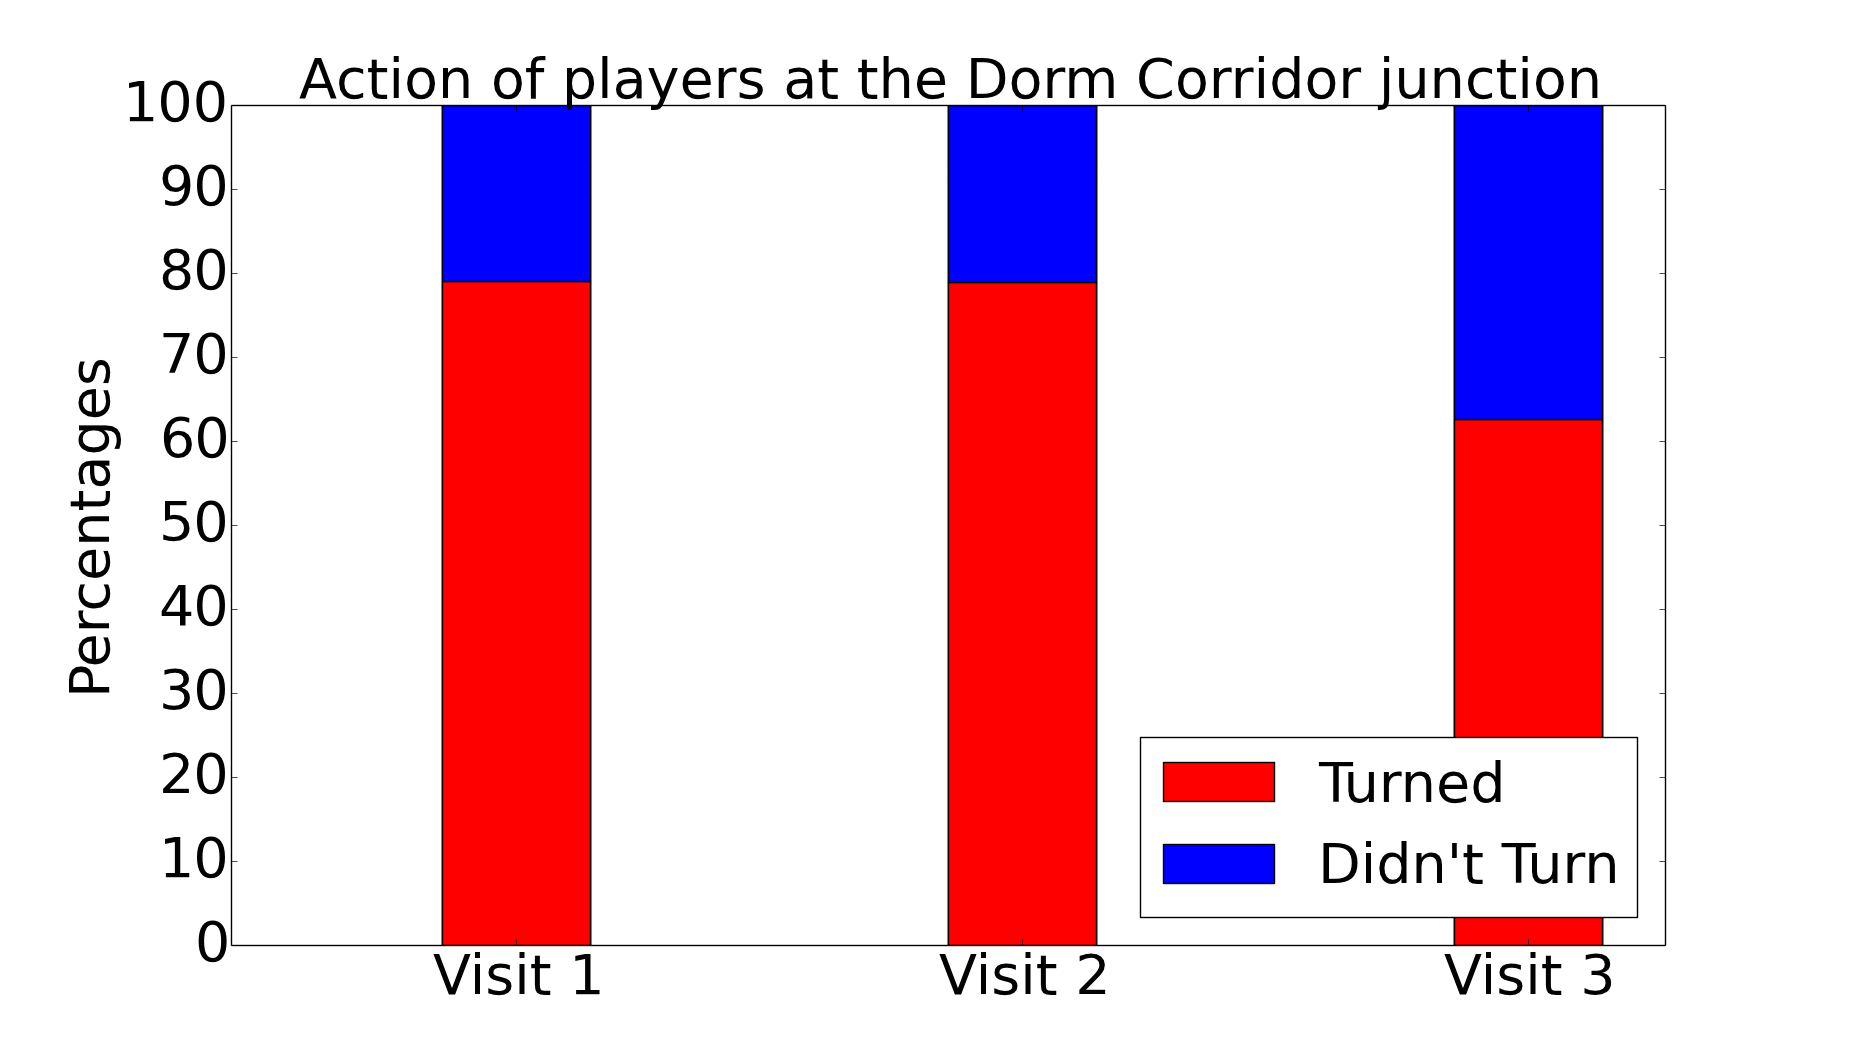
\includegraphics[width=\columnwidth, height=2in]{CorrA2-tasks.png}
    \end{center}
    \caption{Behavior at \emph{junction A2} during tasks}
    \label{fig:junctionA2Behavior}
\end{figure}
\begin{figure}[tb]
    \begin{center}
        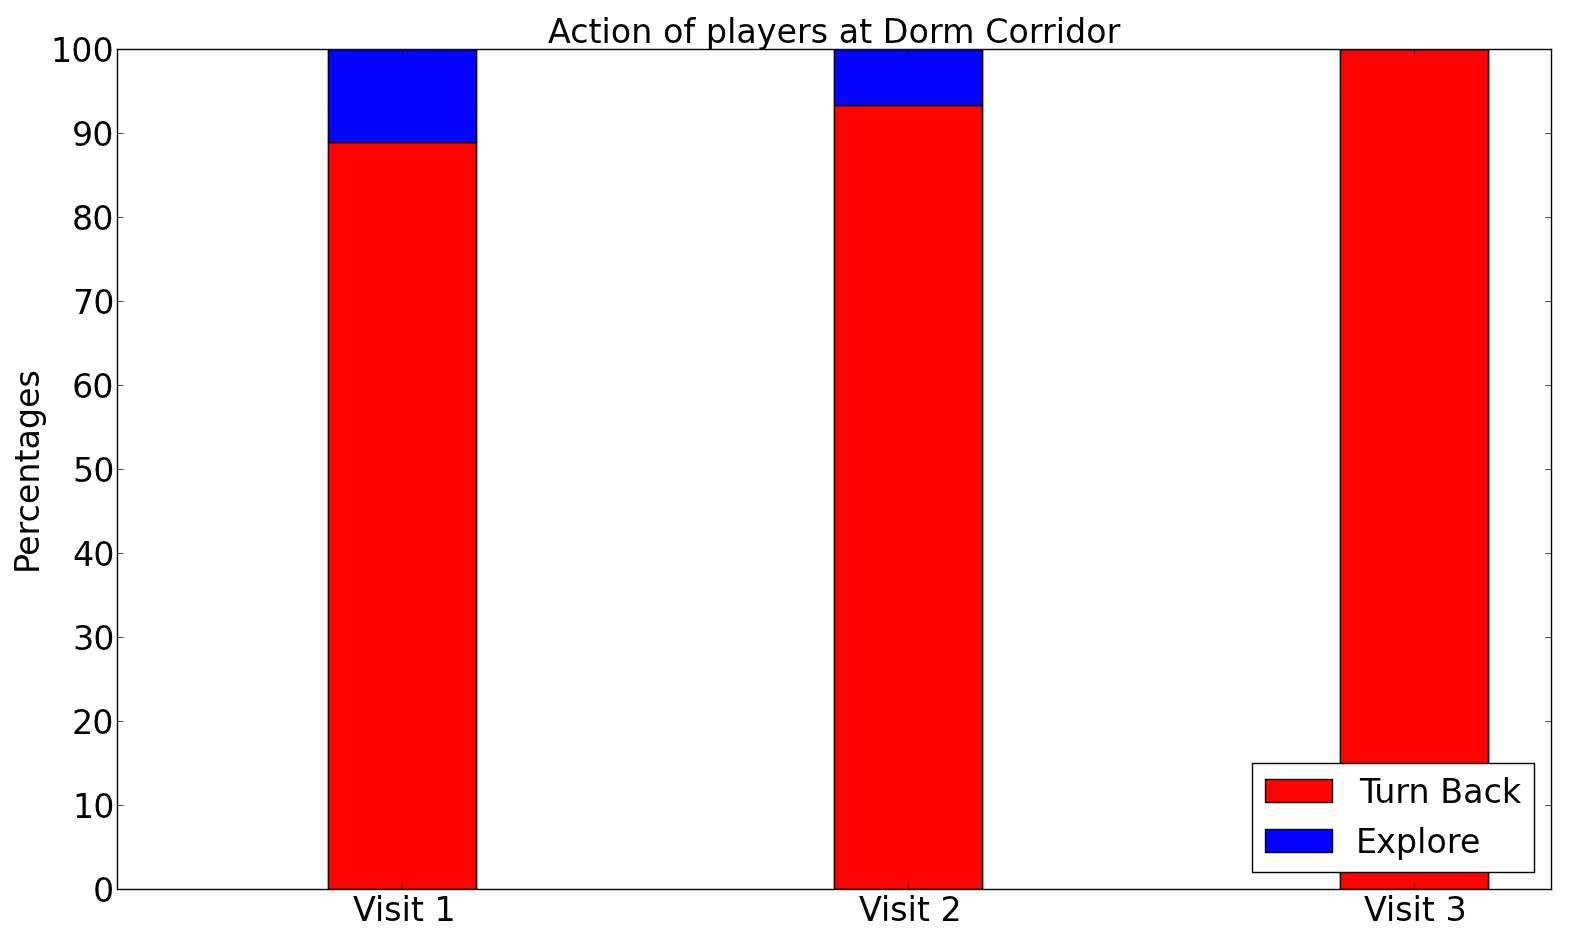
\includegraphics[width=\columnwidth, height=2in]{DormCorr-tasks.png}
    \end{center}
    \caption{Behavior at \emph{Dorm Corridor} during tasks}
    \label{fig:dormCorrBehavior}
\end{figure}

At first this leads to the conclusion that the players never learn and have no memory. However, a similar analysis of movement after entering \emph{Dorm Corridor} indicates that this isn't the case. As shown in Figure~\ref{fig:dormCorrBehavior} indicates that around $80\%$ of the players head right back to the junction after entering this corridor. This probably indicates that the context given by the location of signs and doors in the corridor helps the player remember the corridor, it's location and it's uselessness.



% section empiricalanalysis (end)


% section replicating_the_exploration_behavior (end)

\section{Conclusion} % (fold)
\label{sec:conclusion}

In this paper, we presented a novel game-based methodology that allows for experimental investigation of human navigation and exploration. Although similar methodologies have been used to understand more general crowd behaviour, we believe this is the first case in which quantitative analysis of a game has been used to understand memory in exploration. The Markovian analysis of the players movement in the game revealed a number of significant findings. Firstly, we showed that a simple memory model, with a depth of between 6-8, is sufficient to approximate a `human level' of exploration efficiency. This was consistent in two measure of exploration efficiency, total coverage from a fixed number of hops and the number of hops required to obtain a fixed coverage. The memory depth of 6-8 seems to be consistent with well known studies of human memory capacity. The experiments also highlight the importance of junctions in the exploration process, in particular that decisions (i.e., changing course) seem to almost exclusively occur at junctions. Explorers also try to reduce the number of decisions they have to make by proceeding to the next clearly visible room or corridor if only one such is visible. The results go on to show that people seem to explore environments using a floor-wise strategy, where they are reluctant to move to a different floor until they have finished exploring the current one. Finally, we take particular environmental structures to show that easily recognisable locations can improve exploration efficiency by effectively removing sub-graphs of the room network.

The simple agent-based memory model developed in the paper is shown to approximate human-like efficiency in its exploration strategy. We think this type of simple model is an excellent starting point for developing agent-based models that can be used to evaluate safety-by-design architecture in complex structures. We see the experiments and methods presented here as a starting point for further investigations into the role of exploration and memory in human egress. Similar experiments could be conducted to evaluate the role of long-term memory in exploration, and perhaps validate the three-stage map building of Siegel and White~\cite{Siegel19759}.

%mhl - add the paper which disucsses how people gradually build up different types of map.

% section comparison_and_final_discussion (end)

